The directions that research is taking for visualizing big data are a mix: both applying existing principles such as “details on demand” at higher levels of scale (for example, providing more levels of drill-down between the overview and the lowest level of granularity) and also coming up with new and specialized visualizations that allow larger quantities of data to be represented intelligibly. And as such tools become more sophisticated and more mainstream.
\section{Big Data Visualization Methodology}
Visualizations should be designed in the era of big data in a way such that visualization tools should provide an overview first, then allow zooming and filtering, and provide deeper details on demand.
\subsection{Overview First}
The most important part of a dashboard is the “overview” section. It’s the first thing a viewer sees in the dashboard, and guides the him or her to other parts of the product for further exploration.
\par
The overview should summarize the overarching story from the entire data set without getting into the minor details. It shouldn’t overload the user with too much data, which is where interactive charts, gauges, and maps serve to reduce data clutter, and bring out the story more powerfully
\par
At the same time it shouldn’t leave out important parts of the story by using just a single pie chart, and hiding all the data a layer deeper. Often, great dashboards use a combination of chart types like the line chart, bar chart, maps, and gauges to give the viewer variety, and clarity when studying the data. The overview section should be carefully planned to highlight the important parts of the story, and give lesser weight to the not-so-critical parts. To do this, you may want to organize the entire section into many sub-sections that are clearly labeled. Of course, the important sections would be placed more prominently than the others.
\subsection{Zoom and Filter}
Since all the data is presented to the user in the overview section, the viewer will want to focus on particular areas of interest. This involves zooming and filtering the data using the dashboard’s interactive features: zooming, scrolling, panning, drill-down, legend, range selector, etc. For example, zooming may be drilling down from global to country-specific data while filtering may be excluding information in a specific time range.
\par 
From a design perspective, designer should aim to provide the user with plenty of control for zooming and filtering data from the overview. This will yield maximum insights and action from the information at hand.
\subsection{Details-on-Demand}
Designer have identified areas of interest from the overview section, and have dug deeper into the data using zooming and filtering, but user still may not have found what he started looking for. 
\par 
A dashboard that excels at giving an overview, and allows extensive zooming and filtering, should go all the way and give the viewer access to the minute details. This would bring them as close as possible to the raw data, and equip them to find what they started looking for. This third layer of data would be less visual, and more text-heavy with a focus on accurate information rather than trends. This way the analyst gets what he or she needs, in a way that drives action.
\section{Big Data Visualization Approach}
Visualization can play an important role in using big data to get a complete view of customers. Relationships are an important aspect of many big data scenarios. Social networks are perhaps the most prominent example and are very difficult to understand in text or tabular format; however, visualization can make emerging network trends and patterns apparent. A cloud-based visualization method was proposed to visualize an inherent relationship of users on social network. The method can intentionally present the users’ social relationship based on the correlation matrix to represent a hierarchical relationship of user nodes of social network. In addition, the method uses Hadoop based on cloud for the distributed parallel processing of visualization, which helps expedite the big data of social network
\par 
Big data visualization can be performed through a number of approaches such as more than one view per representation display, dynamical changes in number of factors, and filtering (dynamic query filters, star-field display, and tight coupling).
\subsection{TreeMap}
It is based on space-filling visualization of hierarchical data.
\begin{figure}[h]
	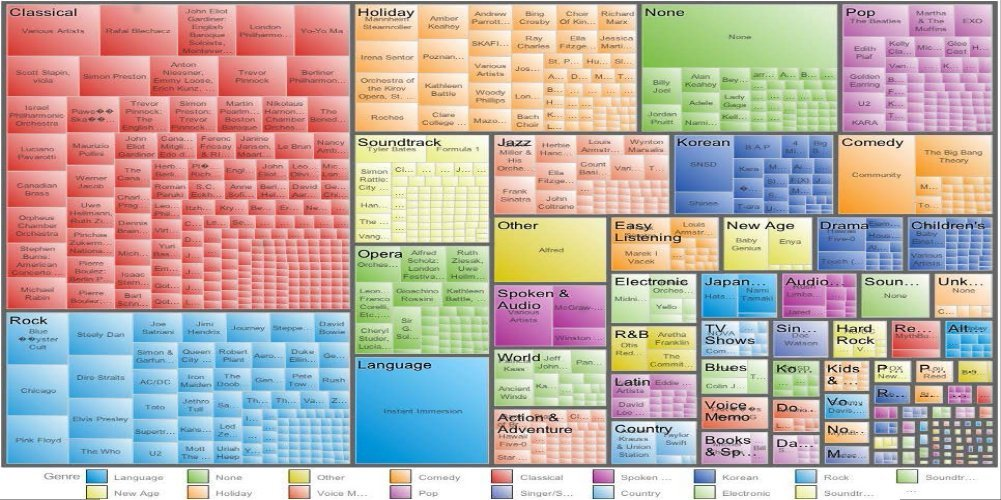
\includegraphics[width=\textwidth, height=8cm]{treemap}
	\centering
	\caption{Treemap}
\end{figure}
\subsection{Parallel Coordinates}
It allows visual analysis to be extended with multiple data factors for different objects.
\begin{figure}[h]
	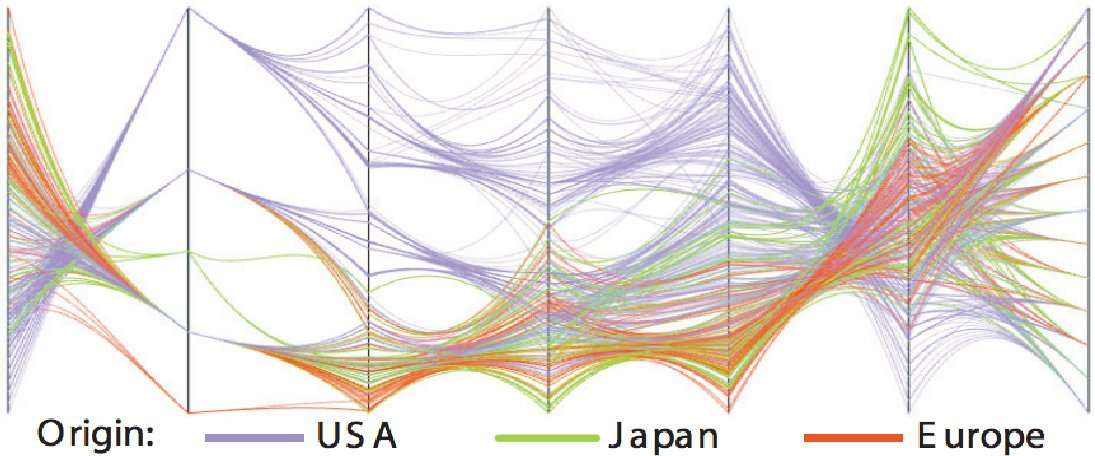
\includegraphics[width=\textwidth, height=5cm]{parallelcoordinates}
	\centering
	\caption{Parallel Coordinates}
\end{figure}
\subsection{Semantic Network}
A semantic network or net is a graph structure for representing knowledge in patterns of 
interconnected nodes and arcs.
\begin{figure}[h]
	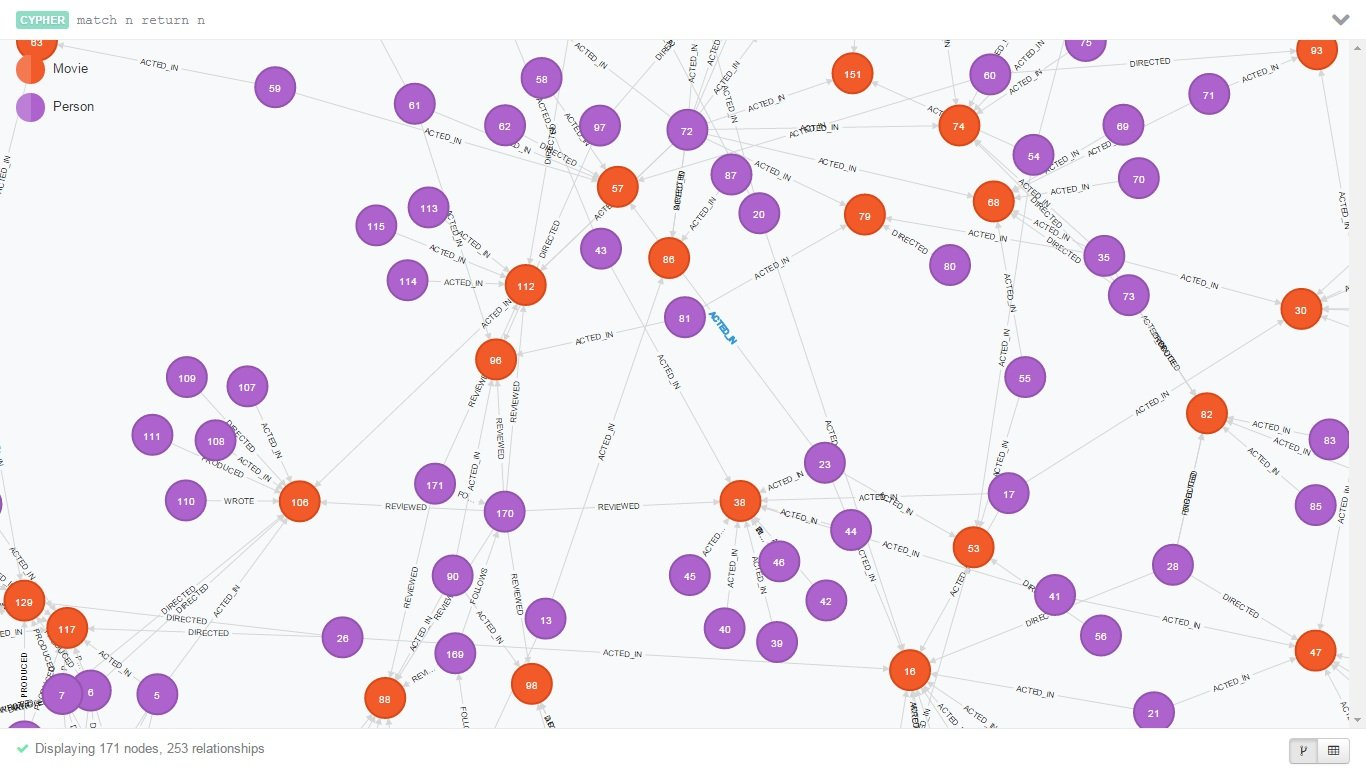
\includegraphics[width=\textwidth, height=6cm]{semanticnetwork}
	\centering
	\caption{Semantic Network}
\end{figure}
\subsection{Sunburst}
It uses tree-map visualization and is converted to polar coordinate system. The main difference is that the variable parameters are not width and height, but a radius and arc length.
\begin{figure}[h]
	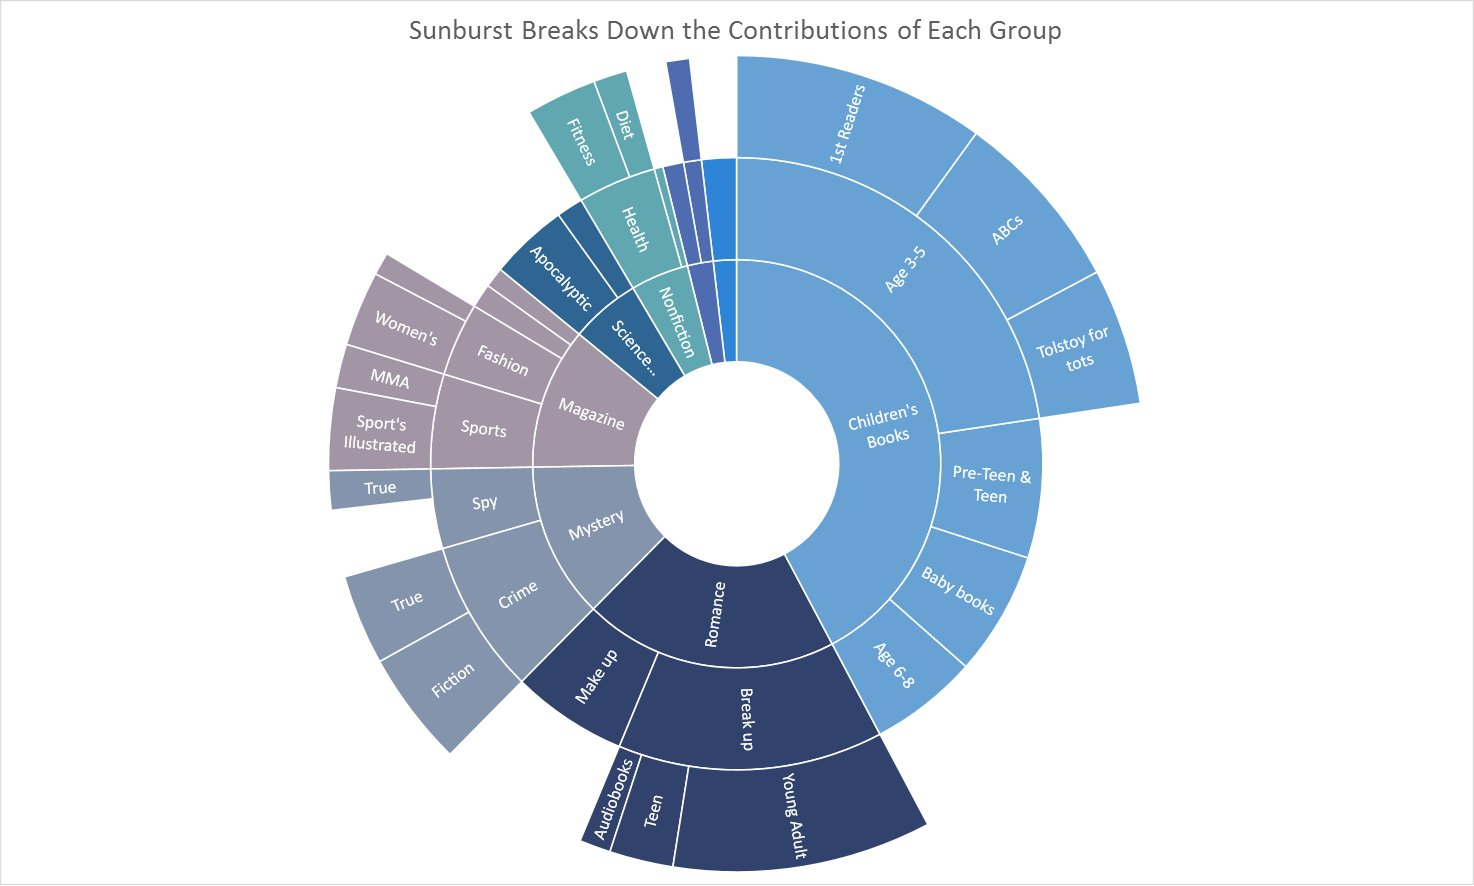
\includegraphics[width=10cm, height=6cm]{sunburst}
	\centering
	\caption{SunBurst Visualization}
\end{figure}
\section{Properties Of Visualization Tools}
Traditional data visualization tools are often inadequate to handle big data. Methods for interactive visualization of big data were presented. First, a design space of scalable visual summaries that use data reduction approaches (such as binned aggregation or sampling) was described to visualize a variety of data types. Methods were then developed for interactive querying (e.g., brushing and linking) among binned plots through a combination of multivariate data tiles and parallel query processing. The developed methods were implemented in imMens, a browser-based visual analysis system that uses WebGL for data processing and rendering on the GPU
\par
Big data processing tools can process ZB (zettabytes) and PB (petabytes) data quite naturally, but they often cannot visualize ZB and PB data. At present, big data processing tools include Hadoop, High Performance Computing and Communications, Storm, Apache Drill, RapidMiner, and Pentaho BI. Data visualization tools include NodeBox, R, Weka, Gephi, Google Chart API, Flot, D3, and Visual.ly, etc. A big data visualization algorithm analysis integrated model based on RHadoop was proposed. The integrated model can process ZB and PB data and show valuable results via visualization. The model is suitable for the design of parallel algorithms for ZB and PB data.
\\
\begin{table}[h!]
\begin{tabular}[h!]{ |p{3cm}||p{3cm}|p{2cm}|p{2.5cm}|}
 \hline
 Method name&Large data volume&Data variety&Data dynamics\\
 \hline
 Treemap&+&-&-\\
 Sunburst&+&-&+\\
 Parallel coordinates&+&+&+\\
 Circular network &+&+&-\\
 Circle packing&+&-&-\\
 \hline
\end{tabular}
\caption{Properties of visualization methods}
\label{table:1}
\end{table}
\section{Virtual Reality Platform for Scientific Data Visualization}
The use of immersive virtual reality (VR) platforms for scientific data visualization has been in the process of exploration including software and inexpensive commodity hardware. These potentially powerful and innovative tools for multi-dimensional data visualization can provide an easy path to collaborative data visualization. Immersion provides benefits beyond traditional “desktop” visualization tools: it results in a better perception of data scape geometry and more intuitive data understanding.
\par
Immersive visualization should become one of the foundations to explore the higher dimensionality and abstraction that are attendant with big data. The intrinsic human pattern recognition (or visual discovery) skills should be maximized through using emerging technologies associated with the immersive VR.
\section{SWOT Analysis Of Current Tools}
The SWOT (Strengths, Weaknesses, Opportunities, and Threats) analysis is a well-known method to ensure that both positive factors and negative factors are identified. A SWOT analysis of the above software tools for big data visualization has been conducted and is shown in table \ref{table:2}. In table \ref{table:2}, Strengths and Opportunities are positive factors; Weaknesses and Threats are negative factors.
\begin{table}[h!]
	\centering
	\begin{tabular}[c]{ |p{6cm}|p{6cm}|}
		\hline
		
		Strengths&Opportunities\\
		\hline
		 With the functions of visualization and interaction for visualizing data.& Immersive visualization with virtual reality (VR) result in a better perception of data scape geometry and more intuitive data understanding.\\
		 \hline
		 Able to visualize a variety of data types&The intrinsic human pattern recognition (or visual discovery) skills
		 could be maximized.\\
		\hline
		\hline
		Weaknesses&Threats\\
		\hline
		There is room to improve in visualizing big data with high velocity or
		the combination of three high Vs (Volume + Velocity + Variety).&Lack adequate visualization in a lot of Big Data applications.\\
		\hline
	\end{tabular}
	\caption{The SWOT analysis of current big data visualization software tools}
	\label{table:2}
\end{table}

